\chapter{Optimizaciones y mejoras del algoritmo \textit{level set} original} 


El algoritmo \textit{level set} es uno de los m\'{a}s utilizados  como consecuencia del buen rendimiento que obtiene al segmentar im\'{a}genes. Existen optimizaciones que lo hacen muy eficiente, como el trabajo que se presentar\'{a} a continuaci\'{o}n \cite{yong1}, que ser\'{a} capaz de satisfacer la demanda que requiere este proyecto.

\

\

\section{Introducci\'{o}n}

Como se ha dado a conocer en el apartado \ref{sec:conclusiones} hay muchos tipos de mejoras y optimizaciones de cada t\'{e}cnica de segmentaci\'{o}n existentes. A la hora de afrontar el problema que el cliente propon\'{i}a se ten\'{i}a que elegir un tipo de segmentaci\'{o}n de las t\'{e}cnicas estudiadas. Entre todas ellas se escogi\'{o} el algoritmo \textit{level set}, por ser un algoritmo de segmentaci\'{o}n eficiente ampliamente utilizado, lo que facilitar\'{i}a la b\'{u}squeda de informaci\'{o}n sobre \'{e}l. Adem\'{a}s, el cliente recomendaba esta t\'{e}cnica, ya que aseguraba que se iban a obtener buenos resultados con ella.

Repasando este algoritmo, las ventajas que tiene son que la segmentaci\'{o}n conseguida es precisa y que no a\~{n}ade sobrecoste al hacer la divisi\'{o}n o uni\'{o}n del contorno. Sin embargo, el algoritmo se basa en la resoluci\'{o}n de ecuaciones diferenciales, lo que supone que el algoritmo sea costoso y lento. Se han desarrollado varias implementaciones en GPU \cite{eri2015}, tambi\'{e}n sobre im\'{a}genes 3D \cite{aaron1}, y en proyectos de fin de carrera tambi\'{e}n se utilizan GPUs \cite{cudaseg} etc. De la misma manera, tambi\'{e}n se han desarrollado paralelizaciones del algoritmo para arquitecturas SMP(\textit{Symmetric Multi-Processing}) \cite{jeon1} o para arquitecturas de memoria distribuida con MPI(\textit{Message Passing Interface})  \cite{moha1}. 

Hay muchos art\'{i}culos sobre este algoritmo, alguna implementaci\'{o}n paralela realizada sobre el algoritmo original y, por lo tanto, a pesar de la paralelizaci\'{o}n, los tiempos que obtienen siguen siendo elevados para las restricciones de este proyecto. Estas paralelizaciones y otras t\'{e}cnicas de optimizaci\'{o}n se centran siempre en resolver las PDEs asociadas a la evoluci\'{o}n del \textit{level set}. Sin embargo, para muchos problemas de imagen, como la segmentaci\'{o}n, no es necesario tanta precisi\'{o}n, ya que el objetivo final es encontrar los bordes de los objetos. En este caso, la evoluci\'{o}n del proceso no tiene tanto inter\'{e}s como el resultado final. Siguiendo esta idea Shi y Karl presentaron un art\'{i}culo muy interesante que ser\'{a} la base de la segmentaci\'{o}n realizada en este proyecto \cite{yong1}.

\

\

\section{Aproximaci\'{o}n a la t\'{e}cnica \textit{level set}}

Como se ha mencionado anteriormente para el objetivo de este proyecto, no se tienen por qu\'{e} resolver las PDEs en el algoritmo \textit{level set} ya que, para una segmentaci\'{o}n, importa m\'{a}s el resultado final que la evoluci\'{o}n propia del algoritmo. Adem\'{a}s, la resoluci\'{o}n de las PDEs conlleva que se tengan que realizar reinicializaciones de la funci\'{o}n de \textit{level set} (representada con la letra $\phi$) lo que implica a\'{u}n m\'{a}s c\'{a}lculo. El trabajo presentado por Shi y Karl \cite{yong1} elimina la reinicializaci\'{o}n al tener una colecci\'{o}n de enteros (los cuales representan la funci\'{o}n $\phi$) que cambian din\'{a}micamente seg\'{u}n va propag\'{a}ndose el contorno y, adem\'{a}s, no calculan las PDEs. Estas dos mejoras elementales hace que su algoritmo sea mucho m\'{a}s r\'{a}pido que el \textit{level set} original. 

En este trabajo se presenta una nueva estrategia de implementaci\'{o}n del m\'{e}todo \textit{level set}. Para el caso de un espacio eucl\'{i}deo de dos dimensiones, una curva C es representada impl\'{i}citamente como el \textit{zero level set} de una funci\'{o}n $\phi$ definida en una cuadr\'{i}cula como se muestra en la figura \ref{aproxLevelSet}. La funci\'{o}n $\phi$ tendr\'{a} un valor negativo dentro de la curva C y un valor positivo fuera de ella, por eso se dice que representa impl\'{i}citamente a la curva C. 

Se definen dos listas de vecindad en esta cuadr\'{i}cula, $L_{in}$ y $L_{out}$. En la imagen se puede ver que el movimiento de la curva C se puede conseguir moviendo un punto de una lista a otra.

Se asume que la funci\'{o}n $\phi$ est\'{a} definida sobre un dominio $D \subset R^k$ y est\'{a} discretizada sobre una rejilla de tama\~{n}o $M_1 \times M_2 \times ... \times M_k$. Estando entonces en una representaci\'{o}n de dos dimensiones, y siguiendo el ejemplo de la rejilla mostrada anteriormente se pueden definir dos listas de vecindad del contorno C: $L_{in}$ y $L_{out}$.

\

$L_{in} = \{x \ | \ \phi(x) < 0$ y $  \exists y \in N(x)$ tal que $\phi(y) > 0\}$

\

$L_{out} = \{x \ | \ \phi(x) > 0$ y $  \exists y \in N(x)$ tal que $\phi(y) < 0\}$

\

\begin{figure}[H]
	\captionsetup{justification=centering}	
	\begin{center}
		\begin{subfigure}[t]{2.5in}
			\centering
			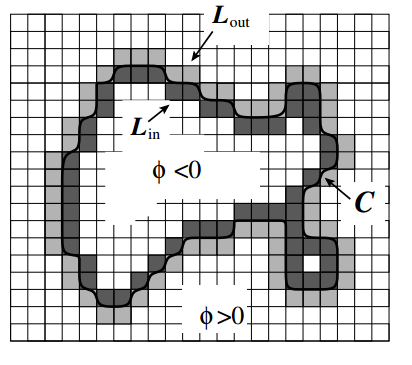
\includegraphics[width=1\textwidth]{./imagenes/aproxLevelSet1}
			\subcaption{}\label{aproxLevelSet1}
		\end{subfigure}
		\begin{subfigure}[t]{2.5in}
			\centering
			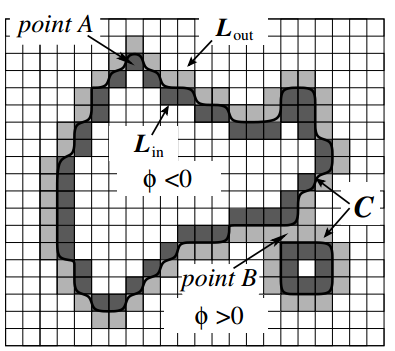
\includegraphics[width=1\textwidth]{./imagenes/aproxLevelSet2}	
			\subcaption{}\label{aproxLevelSet2}
		\end{subfigure}
	\end{center}
	\caption{Representaci\'{o}n de la curva C}
	\vspace{2 mm}		
	\centering
	Fuente: \cite{yong1}	
	\label{aproxLevelSet}
\end{figure}	

Siendo x una coordenada de la rejilla denotada como $x = {x_1,x_2,...,x_k}$ y $N(x)$ como un vecino de x con valor discreto definido como:
\begin{equation}
N(x) = \{y \in D \ | \ \sum_{k=1}^{K} |y_k - x_k| = 1\}  \ \forall x \in D
\end{equation}

Como podemos observar en la figura \ref{aproxLevelSet} la lista $L_{in}$ est\'{a} formada por los puntos de la rejilla que est\'{a}n dentro de la curva C y $L_{out}$ est\'{a} formada por los puntos de la rejilla que est\'{a}n fuera de C. Por lo tanto, como se puede ver en las definiciones formales de las listas, cada punto de ellas tiene que tener un punto vecino de la otra lista, de manera que las dos est\'{e}n "pegadas".

Recordando lo visto en la secci\'{o}n de explicaci\'{o}n del \textit{level set}(\ref{levelSet}) en el cl\'{a}sico \textit{level set} la siguiente PDE es resuelta para evolucionar el contorno C bajo una funci\'{o}n de velocidad F:
\begin{equation}\label{speedLevelSet}
\frac{d\phi}{dt} + F|\nabla \phi| = 0
\end{equation}
La figura \ref{aproxLevelSet2} muestra el proceso evolutivo de la curva C de la figura \ref{aproxLevelSet1}. En el punto marcado como A la curva se ha movido hacia fuera lo que ha modificado el valor de la funci\'{o}n $\phi$ de positivo a negativo. En el punto B la curva se ha movido hacia dentro, partiendo la curva en dos y cambiando el valor de la funci\'{o}n $\phi$ de negativo a positivo. Todo esto tambi\'{e}n ocurre en el \textit{level set} original, con la diferencia de que la resoluci\'{o}n de la PDE mostrada en la ecuaci\'{o}n \ref{speedLevelSet} tiene un coste elevado. Se consiguen los mismos resultados finales f\'{a}cilmente si se usa la relaci\'{o}n entre C, $L_{in}$ y $L_{out}$. Para mover la curva hacia fuera en el punto A de la rejilla tendremos que pasar el punto de la lista $L_{out}$ a $L_{in}$. De manera similar, para mover la curva hacia dentro en el punto B tendremos que cambiar el punto B de $L_{in}$ a $L_{out}$. En general, con aplicar dichas operaciones se va moviendo la curva hacia cualquier punto con el m\'{i}nimo coste operacional. 


\subsubsection{Algoritmo}

Para la realizaci\'{o}n del algoritmo son necesarias estas estructuras:

\begin{itemize}
	\item Un array para la funci\'{o}n de \textit{level set }$\phi$;
	\item Un array para la velocidad (F) con la que se propagar\'{a} la curva;
	\item Dos listas de vecindad de la curva: $L_{in}$ y $L_{out}$.	
\end{itemize}

Nombraremos a los puntos que est\'{a}n dentro de C pero no en la lista $L_{in}$ como <<puntos interiores>> y a los que est\'{a}n fuera de C pero que no pertenecen a $L_{out}$ como <<puntos exteriores>>. Para agilizar a\'{u}n m\'{a}s el c\'{a}lculo, los valores que puede tomar la funci\'{o}n $\phi$ son cuatro enteros: {-3, -1, 1, 3}.
\begin{equation}\label{phi-levelSetEcuation}
\phi (x) = 
\left \{
\begin{array}{rcl}
3 & si & x \mbox{ es un punto exterior} \\
1 & si & x \in L_{out} \\ 
-1 & si & x \in L_{in} \\
-3 & si & x \mbox{ es un punto interior}
\end{array}
\right .
\end{equation}

 Para la funci\'{o}n F de velocidad s\'{o}lo se usa el signo, por lo que tambi\'{e}n es un \textit{array} de enteros con los valores: {1, 0, -1}. En cuanto a las listas, son listas ligadas de manera que la inserci\'{o}n y el borrado de puntos se pueden hacer de manera r\'{a}pida. 
 
 Antes de presentar el algoritmo se aclarar\'{a}n ciertas cuestiones. Para empezar, hay dos operaciones b\'{a}sicas que se utilizan en el algoritmo:
 
 \begin{itemize}
 	\item  La operaci\'{o}n \textit{switch\_in()} para un punto x $\in L_{out}$ se define como:
 	switch\_in(x):
 	\begin{itemize}
 		\item Paso 1: Se quita el punto de $L_{out}$ y se pasa a $L_{in}$. Se cambia el valor de $\phi$ en ese punto: $\phi$(x) = -1.
 		\item Paso 2: Se a\~{n}aden los puntos vecinos de x a $L_{out}$ y se cambian sus respectivos valores en $\phi$. M\'{a}s formalmente: $\forall y$ $\in$ N(x) que satisfaga $\phi(y) = 3$ se a\~{n}ade $y$ a $L_{out}$ y se pone $\phi(y) = 1$
 	\end{itemize}
 	Con esta operaci\'{o}n se mueve el contorno un punto de la rejilla hacia fuera. 
 	\item Similarmente se define la operaci\'{o}n \textit{switch\_out()} para un punto x $\in$ $L_{in}$:
 	 switch\_out(x): 	 
 	 \begin{itemize}
 	 	\item Paso 1: Se quita el punto de  $L_{in}$ y se pasa a $L_{out}$. Se cambia el valor de $\phi$ en ese punto: $\phi$(x) = 1.
 	 	\item Paso 2: Se a\~{n}aden los puntos vecinos de x a $L_{in}$ y se cambia sus respectivos valores en $\phi$. M\'{a}s formalmente: $\forall y $ $\in$ N(x) que satisfaga $\phi(y) = -3$ se a\~{n}ade $y$ a $L_{out}$ y se pone $\phi(y) = -1$
 	 \end{itemize}
 	Con esta operaci\'{o}n se mueve el contorno un punto de la rejilla hacia dentro. 
 \end{itemize}

Por otro lado, la funci\'{o}n F de velocidad presentada antes, normalmente se suele separar en dos velocidades: $F_{ext}$ que depende de los datos y $F_{int}$ para la realizaci\'{o}n de un suavizado del contorno. La velocidad $F_{int}$ es normalmente la curvatura de la curva \cite{chan}. Sin embargo, esta evaluaci\'{o}n de la curva usando la funci\'{o}n $\phi$ suele ser computacionalmente costosa. Tras varios pasos esta funci\'{o}n de velocidad $F_{int}$ puede llegar a ser determinada por un filtro Gaussiano que puede ser aproximado con operaciones con enteros, por lo que se reduce el c\'{o}mputo. Adem\'{a}s, al separar las dos velocidades, no tiene por qu\'{e} hacerse el suavizado despu\'{e}s de cada iteraci\'{o}n de evoluci\'{o}n del contorno como en otros trabajos \cite{yong1}, sino que se realizar\'{a} cuando se satisfaga cierta condici\'{o}n, lo que reduce a\'{u}n m\'{a}s el coste. Con esto entonces, el algoritmo tendr\'{a} dos ciclos principales: el primer ciclo en el que se expandir\'{a} o evolucionar\'{a} el contorno y el segundo ciclo (que se realizar\'{a} de vez en cuando) en el que se suavizar\'{a} el contorno para que se siga expandiendo con normalidad. 


\begin{table}[H]
	\small
	\centering
	\begin{tabular}{|l|}
		\hline		
		\tabitem Paso 1: Inicializar el <<array>> $\phi$, $F_{ext}$ y las dos listas $L_{out}$ y $L_{in}$. \\
		\tabitem Paso 2: Primer ciclo donde se escanean las dos listas para actualizar $\phi$, $L_{out}$ y $L_{in}$. \\
		\quad \quad \quad \quad - Se calcula la velocidad para cada punto de $L_{out}$ y $L_{in}$. \\
		\quad \quad \quad \quad - Evoluci\'{o}n hacia fuera. Recorremos la lista $L_{out}$ y se hace  la operaci\'{o}n \\ 
		\quad \quad \quad \quad \ \ \textit{switch\_in(x)} $\forall x \in L_{out}$ si $F_{ext}$(x) $>$ 0. \\ 
		\quad \quad \quad \quad - Se eliminan los puntos redundantes en $L_{in}$ (v\'{e}ase la figura \ref{switchLevelSet}).\\ 
		\quad \quad \quad \quad \ \ Para ello se tendr\'{a} que recorrer la lista y para cada punto $x \in L_{in}$,\\
		\quad \quad \quad \quad \ \ si $\forall y \in N(x); \phi(y) < 0$, se borra $x$ de $L_{in}$ y se cambia $\phi(x) = -3$. \\ 
		\quad \quad \quad \quad - Evoluci\'{o}n hacia dentro. Recorremos la lista $L_{in}$ y se hace  la operaci\'{o}n \\ 
		\quad \quad \quad \quad \ \ \textit{switch\_out(x)} $\forall x \in L_{in}$ si F(x) $<$ 0. \\ 
		\quad \quad \quad \quad - Se eliminan los puntos redundantes en $L_{out}$. Para ello se tendr\'{a} que \\
		\quad \quad \quad \quad \ \ recorrer la lista y para cada punto $x \in L_{out}$,\\
		\quad \quad \quad \quad \ \ si $\forall y \in N(x); \phi(y) > 0$, se borra $x$ de $L_{out}$ y se cambia $\phi(x) = 3$. \\
		\quad \quad \quad \quad - Se comprueba la condici\'{o}n de parada y si se satisface se continua al paso 3, \\ 
		\quad \quad \quad \quad \ \ si no, seguiremos en el paso 2. \\
		\tabitem Paso 3: Segundo ciclo donde se realiza un suavizado del contorno con un \\ 
		\quad \quad \quad \quad \ \ filtro Gaussiano. \\
		\quad \quad \quad \quad - Evoluci\'{o}n hacia fuera. Recorremos la lista $L_{out}$ y se calcula G $\oplus \ \phi(X)$. \\ 
		\quad \quad \quad \quad \ \ Si  G $\oplus \phi(X) <$ 0 se realiza la operaci\'{o}n \textit{switch\_in(x)} \\ 
		\quad \quad \quad \quad - Se eliminan los puntos redundantes en $L_{in}$ (v\'{e}ase la figura \ref{switchLevelSet}).\\ 
		\quad \quad \quad \quad \ \ Para ello se tendr\'{a} que recorrer la lista y para cada punto $x \in L_{in}$,\\
		\quad \quad \quad \quad \ \ si $\forall y \in N(x); \phi(y) < 0$, se borra $x$ de $L_{in}$ y se cambia $\phi(x) = -3$. \\ 
		\quad \quad \quad \quad - Evoluci\'{o}n hacia dentro. Recorremos la lista $L_{in}$ y se calcula  G $\oplus \ \phi(X)$. \\ 
		\quad \quad \quad \quad \ \ Si G $\oplus \phi(X)$ > 0 se realiza la operaci\'{o}n \textit{switch\_out(x)}  \\ 
		\quad \quad \quad \quad - Se eliminan los puntos redundantes en $L_{out}$. Para ello se tendr\'{a} que \\
		\quad \quad \quad \quad \ \ recorrer la lista y para cada punto $x \in L_{out}$,\\
		\quad \quad \quad \quad \ \ si $\forall y \in N(x); \phi(y) > 0$, se borra $x$ de $L_{out}$ y se cambia $\phi(x) = 3$. \\
		\tabitem Paso 4:  Si se satisface la condici\'{o}n de parada del ciclo uno, se termina el algoritmo, \\
		\quad \quad \quad \quad \ \ si no, se vuelve al paso 2. \\
		\hline
	\end{tabular}
	\caption{Algoritmo completo de la aproximaci\'{o}n del \textit{level set}}
	\vspace{2 mm}		
	Fuente: \cite{yong1}
	\label{algoritmoFastLevelSet}
\end{table}


Aclaradas las cuestiones anteriores, el (r\'{a}pido) algoritmo \textit{level set} \cite{yong1} se muestra en la tabla \ref{algoritmoFastLevelSet}. Como se puede observar el segundo ciclo es pr\'{a}cticamente igual al primer ciclo, a excepci\'{o}n de que la condici\'{o}n de cambiar un punto de una lista a otra, es decir, de hacer una de las operaciones \textit{switch()} que se han explicado anteriormente, depende de un filtro Gaussiano (G) en el segundo ciclo (velocidad $F_{int}$) y de los datos en el primer ciclo (velocidad $F_{ext}$). Las operaciones de \textit{switch\_in()} se realizar\'{a}n cuando el valor de $F$ ($F_{ext}$ en el primer ciclo y $F_{int}$ en el segundo ciclo) sea positivo, que querr\'{a} decir que el contorno deber\'{a} expandirse hacia fuera y las operaciones de \textit{switch\_out()} se realizar\'{a}n cuando el valor de $F$ ($F_{ext}$ en el primer ciclo y $F_{int}$ en el segundo ciclo) sea negativo, contrayendo el contorno en ese punto. V\'{e}ase la figura \ref{switchLevelSet} como ejemplo de expansi\'{o}n del contorno en un p\'{i}xel.

Repasando un poco m\'{a}s el algoritmo \ref{algoritmoFastLevelSet} queda por aclarar las condiciones de parada del algoritmo. As\'{i} pues, el algoritmo se parar\'{a} en el caso de que se cumpla una de estas dos condiciones:

\begin{enumerate}
	\item Que la velocidad $F_{ext}$ de toda la vecindad del contorno cumpla con:
	\begin{enumerate}	
		\item $F(x) \leq 0 \ \forall x \in L_{out}$, es decir, que no se tenga que expandir el contorno por ninguno de sus puntos.
		\item $F(x) \geq 0 \ \forall x \in L_{in}$, es decir, que no se tenga que contraer el contorno en ninguno de sus puntos.
	\end{enumerate}
	\item Que se alcance un determinado n\'{u}mero de iteraciones establecido.
\end{enumerate}
 
Para finalizar, el coste del algoritmo es de orden O(2A($P_1$ + $P_2$)), donde A es el n\'{u}mero de puntos entre el primer contorno creado y el \'{u}ltimo ya evolucionado, $P_1$ y $P_2$ el coste de las operaciones de switch() y el coste que tiene el borrado y la inserci\'{o}n de los puntos en las listas respectivamente. El escalar 2 es debido a que los puntos pueden llegar a pertenecer a una lista primero, y luego a otra, realizando as\'{i} las operaciones dos veces. N\'{o}tese que ese A ser\'{a} mucho menor que la $m \times n$ que ser\'{i}a la anchura (m) por la altura (n) de la imagen, ya que si en la imagen se detectan varios objetos, el tama\~{n}o en puntos o p\'{i}xeles de cada objeto se restar\'{a} a ese $m \times n$.
   
 \begin{figure}[]
 	\captionsetup{justification=centering}
 	\centering
 	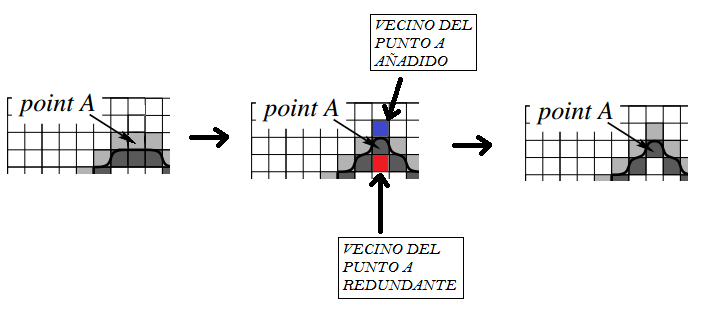
\includegraphics[width=.8\textwidth]{./imagenes/switchLevelSet}
 	\caption{Ejemplo de expansi\'{o}n del contorno un p\'{i}xel hac\'{i}a fuera. Operaciones que se realizan continuamente en el paso 2 y 3 del algoritmo}
	\vspace{2 mm}		
 	Fuente: modificaciones de im\'{a}genes en \cite{yong1}	
 	\label{switchLevelSet}
 \end{figure}
 
 
 
\section{Evoluci\'{o}n del contorno}

Se ha querido a\~{n}adir esta secci\'{o}n para destacar y hablar un poco m\'{a}s en detalle sobre la evoluci\'{o}n de la curva que se ha elegido en esta aproximaci\'{o}n: la presentada en \cite{chan}. Este popular trabajo es conocido como \textit{Chan-Vese model} y a diferencia de como se realizaba la segmentaci\'{o}n, utilizando el uso de detectores de bordes basados en el gradiente, este trabajo realiza la detecci\'{o}n de objetos cuyos bordes no tienen porque estar definidos por el gradiente. Este m\'{e}todo es flexible y potente, capaz de realizar la segmentaci\'{o}n de muchos tipos de im\'{a}genes que con m\'{e}todos tradicionales como \textit{thresholding} o m\'{e}todos basados en el gradiente no pod\'{i}an realizarse. Este m\'{e}todo tambi\'{e}n permite que el contorno se inicialice dentro del objeto o incluso entre el objeto y el fondo ya que el resultado final ser\'{a} siempre el mismo. La figura \ref{chanVese} muestra las posibles inicializaciones. Esta caracter\'{i}stica ser\'{a} de utilidad como se comentar\'{a} en posteriores cap\'{i}tulos.

Para tener una m\'{i}nima idea del avance que esto supuso en la segmentaci\'{o}n de im\'{a}genes, si volvemos a utilizar el buscador \cite{ieee1} y encontramos dicho art\'{i}culo, el n\'{u}mero de citaciones de otros art\'{i}culos registrados en ese explorador alcanza casi la cifra de 2.000, lo que tampoco quiere decir que no haya m\'{a}s trabajos no registrados en \cite{ieee1} que lo citen. 
 
\begin{figure}[H]
	\captionsetup{justification=centering}	
	\begin{center}
		\begin{subfigure}[t]{2.5in}
			\centering
			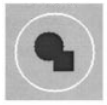
\includegraphics[width=.5\textwidth]{./imagenes/chanVese1}
			\subcaption{}\label{chanVese1}
		\end{subfigure}
		\begin{subfigure}[t]{2.5in}
			\centering
			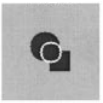
\includegraphics[width=.5\textwidth]{./imagenes/chanVese2}	
			\subcaption{}\label{chanVese2}
		\end{subfigure}
		\begin{subfigure}[t]{2.5in}
			\centering
			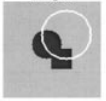
\includegraphics[width=.5\textwidth]{./imagenes/chanVese3}	
			\subcaption{}\label{chanVese3}
		\end{subfigure}
		\begin{subfigure}[t]{2.5in}
			\centering
			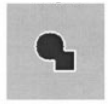
\includegraphics[width=.5\textwidth]{./imagenes/chanVese4}	
			\subcaption{}\label{chanVese4}
		\end{subfigure}
	\end{center}
	\caption{Posibles inicializaciones del contorno con el m\'{e}todo de Chan-Vese}
	\vspace{2 mm}	
	\centering	
 	Fuente: \cite{chan}	
	\label{chanVese}
\end{figure} 